\documentclass[
    aspectratio=169,
    % handout
]{beamer}
% \documentclass[a4paper]{article}
% \usepackage{beamerarticle}

% Setup fonts.
\usepackage{fontspec}
% \setmainfont{Iosevka Etoile}
% \setsansfont{Iosevka Aile}
% \setmonofont{Iosevka}
\setmainfont{CMU Serif}
\setsansfont{CMU Sans Serif}
\setmonofont{CMU Typewriter Text}


%%% Fonts and language setup.
\usepackage{polyglossia}

%% Math
\usepackage{amsmath, amsfonts, amsthm, mathtools} % Advanced math tools.
\usepackage{amssymb}

\usepackage{unicode-math} % Allow TTF and OTF fonts in math and allow direct typing unicode math characters.
\unimathsetup{
    warnings-off={
        mathtools-colon,
        mathtools-overbracket
        }
    }
% \setmathfont{Fira Math}
% \setmathfont{Noto Sans Math}[range = {\Coloneq, cal}]
% \setmathfont{Asana Math}
% [
%         Scale = MatchUppercase,
%         range = {\Coloneq, cal}
% ]
% \setmathfont{STIX Two Math}[range = {\Coloneq, cal}]
% \usepackage{euler-math}
\setmathfont{Lete Sans Math}[CharacterVariant={3,6},StylisticSet={4}]

% \usepackage{emoji}
% \setemojifont{Noto Color Emoji}

\usepackage{booktabs}
% \usepackage{colortbl}
% \usepackage{tabularx}
% \arrayrulecolor{solarizedAccent}
% \newcolumntype{Y}{>{\raggedright\arraybackslash}X}
% \newcolumntype{Z}{>{\raggedleft\arraybackslash}X}

%%% Beamer
% \usetheme{Madrid}
\usetheme{Boadilla}
% \usetheme{Berlin}
% \usecolortheme{solarized}
\usecolortheme{crane}
% \usecolortheme[style=light]{Nord}
% \usefonttheme{Nord}
\setbeamertemplate{navigation symbols}{} %remove navigation symbols
% \setbeamertemplate{headline}{%
%     \begin{beamercolorbox}[ht=2.25ex,dp=3.75ex]{section in head/foot}
%         \insertnavigation{\paperwidth}
%     \end{beamercolorbox}%
% }
\useinnertheme{circles}
% \usefonttheme[stillsansserifsmall,stillsansseriftext]{serif}
% \usepackage{appendixnumberbeamer}
\setbeamertemplate{page number in head/foot}[appendixframenumber]
%% Use with Solarized theme
% \setbeamercolor{author in head/foot}{fg=solarizedRebase03}
% \setbeamercolor{title in head/foot}{fg=solarizedRebase03}
% \setbeamercolor{date in head/foot}{fg=solarizedRebase03}
% \setbeamercolor{page number in head/foot}{fg=solarizedRebase03}

%%% Misc

\setdefaultlanguage{russian}
\setotherlanguage{english}

\uselanguage{russian}
\languagepath{russian}
\newtranslation[to = russian]{Definition}{Определение}
\newtranslation[to = russian]{definition}{определение}
\newtranslation[to = russian]{Theorem}{Теорема}
\newtranslation[to = russian]{theorem}{теорема}

%% Tikz
% \usepackage{tikz}
% \usetikzlibrary{arrows.meta}
% \usetikzlibrary{external}
% \usetikzlibrary{positioning}
% \usetikzlibrary{shapes.geometric}
% \usetikzlibrary{automata}
% \usetikzlibrary{decorations.pathmorphing}
% \usetikzlibrary{calc}
% \tikzsetexternalprefix{figures/}
% \tikzexternalize

\usepackage{xurl}

%% Pictures
\usepackage{graphicx}
\graphicspath{{figures/}}

%%% Code
\usepackage[newfloat]{minted}
% \usemintedstyle{solarized-light}
\usemintedstyle{emacs}
% \SetupFloatingEnvironment{listing}{name=Листинг}

\usepackage{ebproof}

\usepackage[backend=biber, style=alphabetic]{biblatex}
\renewcommand*{\bibfont}{\footnotesize}
% \addbibresource{rewriting-and-deforestation.bib}

\usepackage{csquotes}
\usepackage{hyperref}

\title{Введение в OpenCL}
\author{Николай Пономарев}
\institute[Матмех СПбГУ]{Математико-механический факультет СПбГУ}
\date{10 апреля 2025 г.}

\begin{document}

\begin{frame}[plain, noframenumbering]
    \maketitle
\end{frame}

\begin{frame}
    \frametitle{OpenCL}

    \begin{itemize}
        \item OpenCL (Open Computing Language) for \textbf{Parallel} Programming of \textbf{Heterogeneous} Systems
        \item Один из стандартов The Khronos Group~--- консорциума, который занимается разработкой открытых стандартов в областях параллельных вычислений, машинного обучения, компьютерной графики
              \begin{itemize}
                  \item Насчитывает более 180 организаций-участников
                  \item Поддерживает 21 стандарт, среди них Vulkan, OpenGL, OpenCL, SPIR-V, WebGL
              \end{itemize}
        \item Можно найти в девайсах от AMD, Arm, Google, Imagination Technologies, Intel, NVIDIA, Qualcomm, ...
        \item Используется в OpenCV, FFmpeg, ViennaCL, GNU Octave, Matlab, ...
    \end{itemize}

\end{frame}

\begin{frame}
    \frametitle{Параллелизм по данным}

    \begin{itemize}
        \item Можем применить функцию к различным элементам коллекции независимо\footnote{Картинка из \url{https://github.com/YaccConstructor/articles/tree/master/2025/GPGPU_OpenCL_Intro}}
              \begin{center}
                  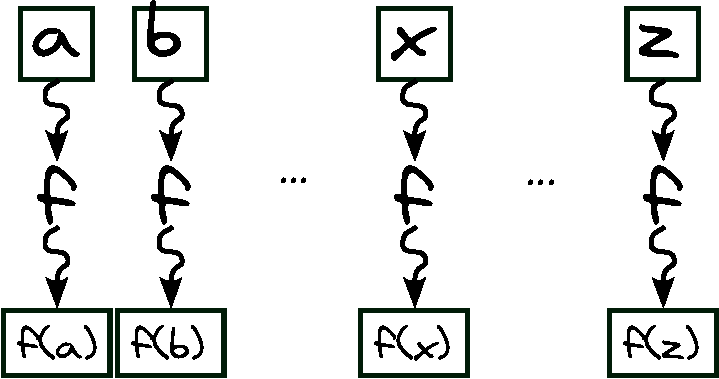
\includegraphics[height=3cm]{simd_crp.pdf}
              \end{center}
        \item Single Instruction Multiple Data (SIMD)~--- реализация параллелизма по данным на уровне процессора
              \begin{itemize}
                  \item Инструкция $\Rightarrow$ действия более простые и гранулярные
                  \item Данные должны быть однородны
              \end{itemize}
        \item Хорошо подходит для решения задач линейной алгебры и обработки изображений
              %   \begin{itemize}
              %       \item Умножений матриц
              %       \item Свёрточные фильтры
              %   \end{itemize}
    \end{itemize}

\end{frame}

\begin{frame}
    \frametitle{Устройства, где работает OpenCL}

    \begin{itemize}
        \item Central Processing Unit, CPU
        \item Graphics Processing Unit, GPU
        \item Digital Signal Processor, DSP
        \item Field-Programmable Gate Array, FPGA
        \item Tensor Processor
        \item ...
    \end{itemize}

\end{frame}

\begin{frame}
    \frametitle{Версии OpenCL}

    \begin{description}
        \item[\textbf{1.0}] Первый релиз, 2008 г.
        \item[\textbf{1.2}] Baseline для современного оборудования, 2011 г.
        \item[\textbf{2.x}] Крупное обновление, но откатили в 3.0, 2013--2017 г.
        \item[\textbf{3.0}] База из 1.2 и расширения по усмотрению производителя, 2020 г.
    \end{description}
    \vspace{1em}
    Khronos часто показывает в примерах код для 2.x~--- но устройства почти не поддерживают эти версии!

    \vspace{1em}
    Обычно в пользовательских устройствах можно найти либо 1.2, либо 3.0
\end{frame}

\begin{frame}
    \frametitle{Структура программы}

    \begin{columns}[T]
        \begin{column}{0.7\textwidth}
            \begin{itemize}
                \item Программа исполняется на двух устройствах: хосте и ускорителе
                \item Хост (host)~--- обычно CPU устройства
                      \begin{itemize}
                          \item Отвечает за общение с внешним миром, подготовку данных и запуск кода на девайсе
                          \item Можно использовать привычный язык программирования
                      \end{itemize}
                \item Ускоритель (девайс, device)~--- вычислительные модули, поддерживающие OpenCL
                      \begin{itemize}
                          \item Исполняет код по просьбе хоста
                          \item Язык программирования \enquote{прибит}
                          \item Программу обычно называют \enquote{ядром} (kernel)
                      \end{itemize}
            \end{itemize}
        \end{column}
        \begin{column}{0.3\textwidth}
            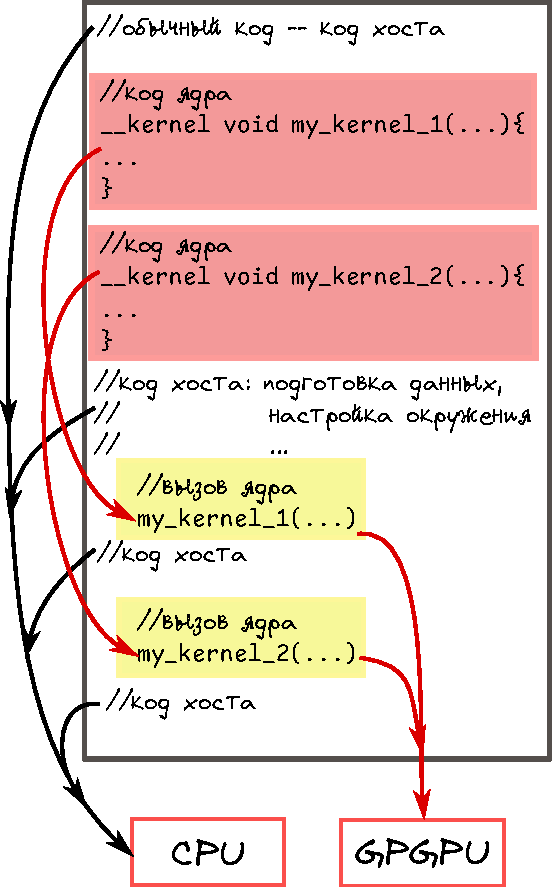
\includegraphics[width=0.9\linewidth]{host-kernel-code.pdf}
        \end{column}
    \end{columns}
\end{frame}

\begin{frame}
    \frametitle{Взаимодействие хоста и ускорителя}

    \begin{itemize}
        \item Обнаружение, подключение и конфигурация устройств
        \item Работа с памятью
              \begin{itemize}
                  \item Выделение/освобождение
                  \item Контроль доступа и синхронизация между хостом и ускорителем
                  \item Основной примитив~--- буфер, но с 2.0 поддерживается и Shared Virtual Memory (SVM)
              \end{itemize}
        \item Выполнение команд
              \begin{itemize}
                  \item Передача данных, запуск ядер, синхронизация
                  \item Основной интерфейс взаимодействия~--- очередь команд
                        \begin{itemize}
                            \item Неблокирующая: центральный процессор ставит задачи, но не дожидается их исполнения
                            \item Нужны дополнительные действия чтобы узнать, когда закончилась определённая задача
                            \item In-order: команды выполняются строго друг за другом
                            \item Может быть out-of-order
                            \item Синхронизация между несколькими очередями возможна, но требует отдельной работы
                        \end{itemize}
              \end{itemize}
    \end{itemize}

\end{frame}

\begin{frame}
    \frametitle{Языки программирования}

    \begin{columns}[t]
        \begin{column}{0.5\textwidth}
            Языки программирования хоста:
            \begin{itemize}
                \item \textbf{C}
                \item \textbf{C++}
                \item Python\footnote[frame]{PyOpenCL: \url{https://documen.tician.de/pyopencl/}}
                \item Rust\footnote[frame]{ocl: \url{https://github.com/cogciprocate/ocl}}
                \item Julia\footnote[frame]{OpenCL.jl: \url{https://github.com/JuliaGPU/OpenCL.jl}}
                \item ...
            \end{itemize}
        \end{column}
        \begin{column}{0.5\textwidth}
            Языки программирования ускорителя:
            \begin{itemize}
                \item \textbf{The OpenCL C Kernel Language}
                \item C++ for OpenCL
            \end{itemize}
        \end{column}
    \end{columns}

\end{frame}

\begin{frame}
    \frametitle{The OpenCL C Kernel Language}

    \begin{itemize}
        \item Диалект C99: специальные типы данных (векторы, изображения, очереди команд), модификаторы памяти (глобальная, локальная, константная, приватная)
        \item Online компиляция, но можно и offline
        \item Собственный stdlib
        \item Расширения
              \begin{itemize}
                  \item Предусмотренные cтандартом: \texttt{cl\_khr\_fp64, cl\_khr\_int64\_extended\_atomics, ...}
                  \item Расширения от вендоров: \texttt{cl\_nv\_pragma\_unroll, cl\_amd\_fp64, ...}
              \end{itemize}
    \end{itemize}

\end{frame}

\begin{frame}
    \frametitle{Пример 1}

    См. директорию \texttt{cpp\_vadd\_example}

\end{frame}

\begin{frame}
    \frametitle{Параллельность}

    \begin{columns}[T]
        \begin{column}{0.5\textwidth}
            \begin{itemize}
                \item Виртуальная решётка (\textbf{NDRange}) \enquote{потоков} (\textbf{work-items})
                      \begin{itemize}
                          \item одно-, двух-, трёхмерная
                          \item Группировка узлов в рабочие группы (\textbf{work-group}) фиксированного размера
                          \item Возможность получить глобальные и локальные координаты \enquote{потока}
                      \end{itemize}
                \item Параметры (размеры) решётки связаны с \enquote{размерами} обрабатываемых данных
            \end{itemize}
        \end{column}
        \begin{column}{0.5\textwidth}
            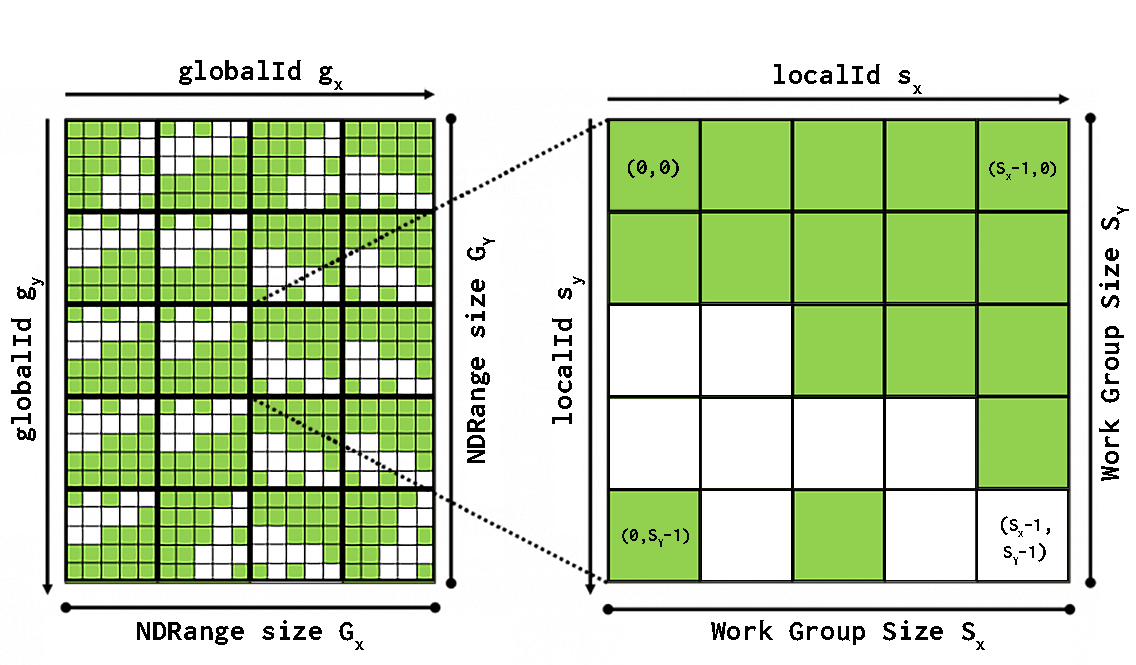
\includegraphics[width=\linewidth]{opeclmap4.png}
        \end{column}
    \end{columns}

\end{frame}

\begin{frame}
    \frametitle{Модель памяти}

    \begin{columns}[T]
        \begin{column}{0.5\textwidth}
            Память в OpenCL выстраивается в иерархию:
            \begin{itemize}
                \item Память хоста~--- не доступна потокам напрямую
                \item Глобальная/константная память~--- доступна в любой части ускорителя
                \item Локальная~--- доступна группе \enquote{потоку}
                \item Приватная~--- доступна только \enquote{потоку}
            \end{itemize}
            Управление памятью ручное.
            Перемещение и синхронизация осуществляются явно, по команде программиста.
        \end{column}
        \begin{column}{0.5\textwidth}
            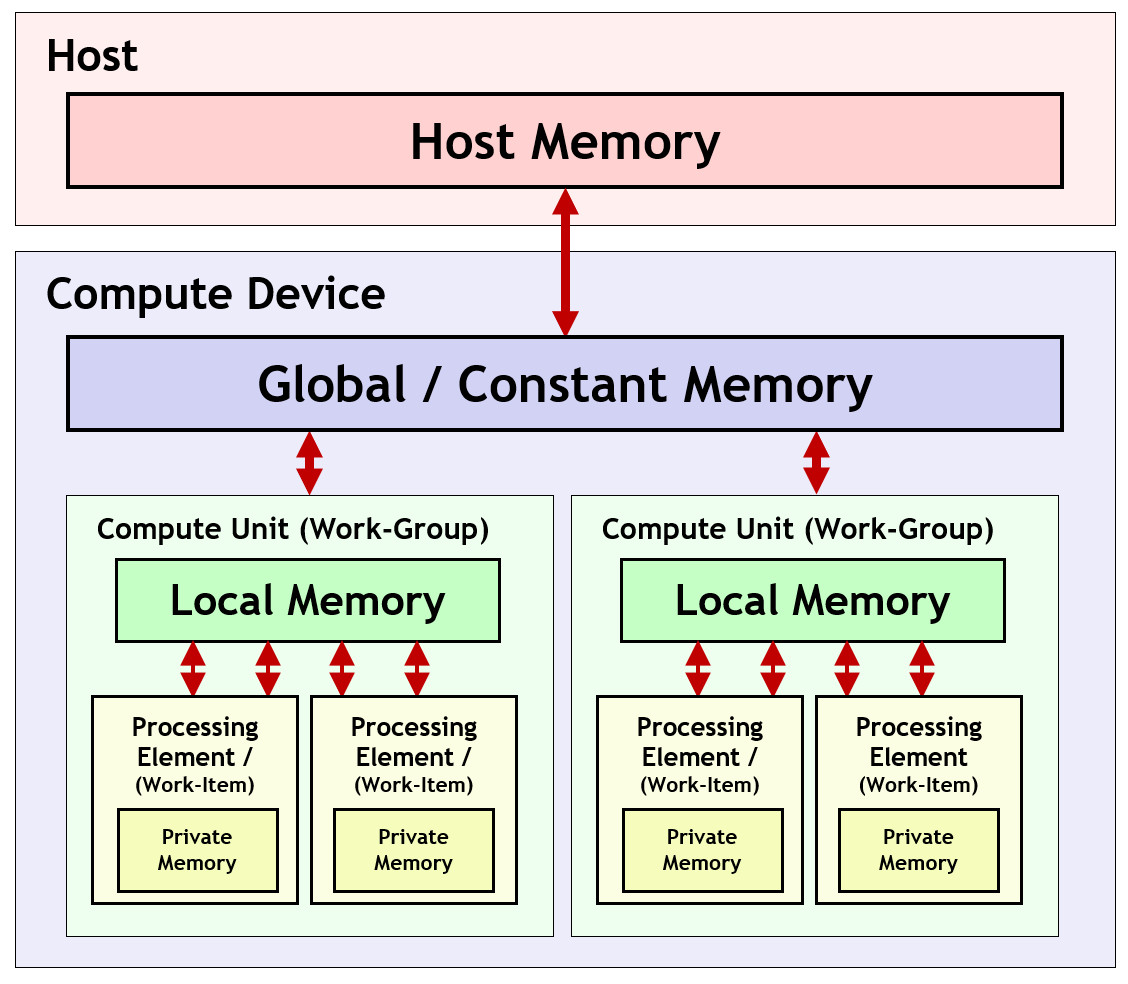
\includegraphics[width=\linewidth]{memory_model.jpg}
        \end{column}
    \end{columns}

\end{frame}

\begin{frame}
    \frametitle{Пример 2}

    См. \texttt{myGEMM/src/kernels.cl}, ядро \texttt{myGEMM2}

    И пояснения из \url{https://cnugteren.github.io/tutorial/pages/page4.html}

\end{frame}

\begin{frame}
    \frametitle{Работа с изображениями}

    \begin{itemize}
        \item OpenCL поддерживает изображения на уровне типов
        \item Для работы с ними имеются соответствующие API
        \item Информация о формате и размере изображения передаётся при загрузке в память
        \item Внутри ядра необходимо использовать сэмплеры~--- объекты, которые описывают, как извлекаются элементы изображения
              \begin{itemize}
                  \item какая используется координатная система (целочисленные или нормализованные координаты)
                  \item как обрабатывается ситуация выхода координат за пределы изображения (обнуление или установка «цвета» ближайшего элемента
                  \item производится ли интерполяция при извлечении значений, расположенных «между» элементами изображения
              \end{itemize}
    \end{itemize}

\end{frame}

\begin{frame}
    \frametitle{Пример 3}

    См. директорию \texttt{cpp\_gaussian\_filter\_example}

\end{frame}

\begin{frame}
    \frametitle{Продвинутые возможности}

    \begin{itemize}
        \item Интеграция OpenCL и OpenGL
        \item Offline компиляция ядер
        \item Асинхронность
        \item Использование нескольких устройств
    \end{itemize}

\end{frame}

\begin{frame}
    \frametitle{Полезные ссылки}

    \begin{itemize}
        \item Презентация Григорьева С. В.
              \begin{itemize}
                  \item \scriptsize{\url{https://github.com/YaccConstructor/articles/blob/master/2025/GPGPU_OpenCL_Intro/SemyonGrigorev_YWS_GPU_OpenCL.pdf}}
              \end{itemize}
        \item {Khronos OpenCL}
              \begin{itemize}
                  \item \scriptsize{\url{https://www.khronos.org/opencl/}}
              \end{itemize}
        \item {Курс по разработке под GPGPU от EuroCC National Competence Center Sweden}
              \begin{itemize}
                  \item \scriptsize{\url{https://enccs.github.io/gpu-programming/}}
              \end{itemize}
        \item {Cornell University, Understanding GPU Architecture}
              \begin{itemize}
                  \item \scriptsize{\url{https://cvw.cac.cornell.edu/gpu-architecture}}
              \end{itemize}
        \item {Антонюк В. А. OpenCL Открытый язык для параллельных программ, учебное пособие, 2017.}
              \begin{itemize}
                  \item \scriptsize{\url{https://istina.msu.ru/publications/book/76785028/}}
              \end{itemize}
        \item Tutorial: OpenCL SGEMM tuning for Kepler
              \begin{itemize}
                  \item \scriptsize{\url{https://cnugteren.github.io/tutorial/pages/page1.html}}
              \end{itemize}
        \item OpenCL Programming Guide 1.2 Examples
              \begin{itemize}
                  \item \scriptsize{\url{https://github.com/bgaster/opencl-book-samples}}
              \end{itemize}
    \end{itemize}

\end{frame}

\begin{frame}
    \frametitle{Вопросы к экзамену}

    \begin{enumerate}
        \item OpenCL: общие сведения, поддерживаемый вид параллелизма, поддерживаемые устройства, языки программирования
        \item OpenCL: структура программы, взаимодействие хоста и ускорителя, рабочие группы и модель памяти
    \end{enumerate}

\end{frame}

\end{document}
